\subsection{\labeltext[UC01 - Acesso ao sistema]{UC1.1 - Criar Conta}{uc:11}}
A imagem identificada como figura~\ref{fig:chap211} apresenta o diagrama de caso de uso \ref{uc:11} e tem como objetivo apresentar as interações entre os atores e o sistema.

\vspace*{5mm}

\begin{figure}[H]
	\centering
	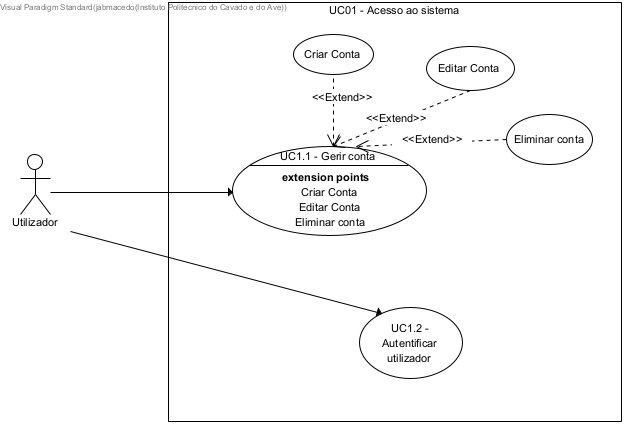
\includegraphics[width=1\linewidth]{./img/Diagramas\_UC/UC01.jpg}  % largura percentual 
	\caption{\ref{uc:11}}
	\label{fig:chap211}
\end{figure}

\noindent \textbf{Descrição} \\
\textbf{ID:} UC1.1 \\  
\textbf{Nível de importância:} Alta \\
\textbf{Nome:} Criar Conta \\
\textbf{Ator principal:} Utilizador \\
\textbf{Atores secundários:} --------- \\
\textbf{Breve descrição:} O utilizador para usar a aplicação deve criar conta. \\ 
\textbf{Ativador:} Iniciar a aplicação.  \\
\textbf{Pré-condições:} --------- \\
\textbf{Fluxo normal dos eventos:} \\
1. Abrir aplicação  \\
2. Clicar em registo de conta. \\
3. Preencher dados. \\
4. Carregar no botão "Registar"  \\
\textbf{Sub-fluxos:} --------- \\
\textbf{Fluxos alternativos/excecionais:}  \\
1. Erro de insersão de dados. \\

\subsection{UC1.2 - Autenticar utilizador}
\vspace*{5mm}

\noindent \textbf{Descrição} \\
\textbf{ID:} UC1.2 \\  
\textbf{Nível de importância:} Alta \\
\textbf{Nome:} Autenticar utilizador \\
\textbf{Ator principal:} Utilizador \\
\textbf{Atores secundários:} --------- \\
\textbf{Breve descrição:} O utilizador para usar o sistema deverá introduzir os dados de autenticação. A autenticação é validada com os dados da base de dados do sistema inseridos no ato da criação de conta. \\ 
\textbf{Ativador:} Utilizador autenticar-se.  Dados do utilizador registados na base de dados do sistema. \\
\textbf{Pré-condições:} Ter conta criada. \\
\textbf{Fluxo normal dos eventos:} \\
1. Abrir o sistema.  \\
2. Inserir email. \\
3. Inserir palavra-chave. \\
4. Carregar no botão "Login"  \\
\textbf{Sub-fluxos:} --------- \\
\textbf{Fluxos alternativos/excecionais:}  \\
1. Erro de autenticação, email ou palavra-chave incorretas. \\